\documentclass[10pt,twoside]{article}

\usepackage[T1]{fontenc}
\usepackage[scaled]{uarial}
\renewcommand{\familydefault}{\sfdefault}
\usepackage{caption}
\captionsetup[figure]{name=Figura}
\captionsetup[table]{name=Tabella}
\usepackage{tgadventor}
\usepackage{xcolor}
\definecolor{darkblue}{rgb}{0,0,0.4}
\usepackage[ocgcolorlinks]{hyperref}
\hypersetup{
  colorlinks=true,      % usa il colore invece delle cornici
  linkcolor=darkblue,       % colore dei link interni
  citecolor=darkblue,       % colore delle citazioni
  urlcolor=darkblue,        % colore degli URL
  pdfborder={0 0 0},    % niente cornici
  pdfhighlight=/I       % inverti al rollover (schiarisce leggermente)
}
\usepackage{amsfonts}
\usepackage{amssymb}
\usepackage{tabularx}
\usepackage{amsmath}
\usepackage{listings}
\usepackage{float}
\usepackage[table,xcdraw]{xcolor}
\usepackage{array}
\usepackage[margin=2.54cm]{geometry}
\usepackage{fancyhdr}
\usepackage{graphicx}
\usepackage{titlesec}
\usepackage{setspace}
\usepackage{parskip}
\usepackage{lmodern}
\pagenumbering{gobble}  % disabilita completamente la numerazione visibile



\begin{document}

\begin{titlepage}
    \centering
    
\includegraphics{img/logo.png}\par\vspace{1cm}
    {\scshape\Large Università degli Studi di Padova \par}
    \vspace{1.5cm}
    {\scshape\large Dipartimento di Matematica\par}
    \vspace{0.5cm}
    {\scshape\large Laurea Triennale in Informatica\par}
    \vspace{2cm}
    {\scshape\Large Progetto di Basi di Dati\\\par}
    \vspace{1cm}
    \hrule
    \vspace{1cm}
    {\large\bfseries
    Basi di Dati di un Sistema Informativo\\
    per la Gestione di una Scuola Guida\par}
    \vspace{1cm}
    \hrule
    \vfill
    {\large Andrea Difino, Davide Colabove\par}
\end{titlepage}

\pagestyle{fancy}
\fancyhead{}
\fancyhead[C]{\fontsize{9}{9}\selectfont Progetto di una Base di Dati di un Sistema Informativo per la Gestione Scuola Guida}
\title{\fontsize{12}{12}\selectfont \textbf{A.A. 2024/25} \\ Corso di Laurea in Scienze e Tecnologie Informatiche SC1167}
\date{}
\maketitle

\renewcommand{\contentsname}{Indice}
\tableofcontents

\newpage
\clearpage
\pagenumbering{arabic}
\section{Abstract}{
    Questo lavoro sviluppa una base di dati progettata per gestire in modo strutturato e coerente le informazioni relative alle scuole guida, agli istruttori, agli iscritti ai corsi e agli esami sostenuti dagli allievi. 
    
    L’obiettivo principale è fornire un sistema che supporti le attività di pianificazione, monitoraggio e ottimizzazione delle risorse didattiche, garantendo un accesso organizzato ai dati e facilitando la loro analisi.

    Nel contesto della formazione alla guida, la base di dati proposta distingue tra lezioni teoriche e pratiche, gestendo attributi specifici quali assegnazione di aule, veicoli disponibili e disponibilità degli istruttori. Gli iscritti sono tracciati in base ai percorsi di formazione intrapresi e ai risultati degli esami, con particolare attenzione alle performance nelle prove teoriche e pratiche. Il sistema registra anche le prenotazioni delle lezioni e i pagamenti associati ai servizi offerti.

    Questa base di dati è progettata per garantire un’archiviazione efficiente e strutturata delle informazioni formative, migliorando il recupero e l’analisi dei dati. L’organizzazione sistematica delle informazioni contribuisce a un utilizzo più efficace delle risorse didattiche, ottimizzando la gestione delle scuole guida e supportando i processi decisionali.

}

\section{Analisi dei Requisiti}{
    \label{sec:analisiRequisiti}
    Questa sezione riassume i requisiti a cui deve sottostare la base di dati.

    \paragraph{Iscritto.}
    Gli iscritti sono le persone che frequentano i corsi della scuola guida e sono identificati attraverso:

    \begin{itemize}
        \item Codice Fiscale (identificativo univoco).
        \item Nome.
        \item Cognome.
        \item Numero di telefono.
        \item Indirizzo email.
        \item Città (CAP, Nome, Provincia) e indirizzo di residenza.
        \item Categoria di patente richiesta (A, B, C, ecc.).
        \item Data di iscrizione.
    \end{itemize}
    
    Ogni iscritto può partecipare a più lezioni teoriche e pratiche, sostenere più esami, e può lasciare recensioni su lezioni o istruttori. \\
    Abbiamo scelto di implementare l'attributo CAP perché esistono cittá distinte ma con lo stesso CAP (es. Terrassa Padovana, Pernumia, Albignasego, Pozzonovo che ricadono tutte sotto il CAP 35020) ma al contempo anche cittá (es. Padova, Roma, Milano) con piu' CAP al loro interno.
    

    \paragraph{Istruttore.}
    Gli istruttori sono i docenti responsabili delle lezioni e sono descritti tramite:
    
    \begin{itemize}
        \item Codice Fiscale (identificativo univoco).
        \item Nome.
        \item Cognome.
        \item Numero di telefono.
        \item Indirizzo email.
        \item Anni di esperienza professionale.
        \item Categorie di patente per cui sono abilitati all’insegnamento.
    \end{itemize}

    Un istruttore può tenere più lezioni sia teoriche che pratiche, ma non può essere assegnato contemporaneamente a due lezioni sovrapposte.
    

    \paragraph{Patente.}
    Le Patenti determinano per cosa gli istruttori sono abilitati ad insegnare:
    
    \begin{itemize}
        \item TipoPatente.
        \item Descrizione.
    \end{itemize}

    Un istruttore può essere abilitato ad insegnare più patenti, ma una patente può non essere insegnata da nessun istruttore.

    \paragraph{Veicolo.}
    I veicoli sono utilizzati per le lezioni pratiche e per gli esami pratici. Per ogni veicolo vengono registrate le seguenti informazioni:
    
    \begin{itemize}
        \item Targa (identificativo univoco).
        \item Modello.
        \item Tipo di veicolo (Auto, Moto, ecc.).
        \item Anno di immatricolazione.
        \item Stato operativo (disponibile, in manutenzione, non disponibile).
    \end{itemize}

    Ogni veicolo può essere utilizzato in più lezioni pratiche o esami pratici. Tuttavia, ogni lezione pratica o esame pratico è associato a un solo veicolo alla volta.
    

    \paragraph{Aula.}
    Le aule sono gli spazi in cui si svolgono le lezioni teoriche e sono caratterizzate da:

    \begin{itemize}
        \item Nome aula. (identificativo univoco)
        \item Numero di posti disponibili.
        \item Tipologia di attrezzatura didattica disponibile (proiettore, lavagna, ecc.).
    \end{itemize}

    Un’aula può ospitare più lezioni, ma non contemporaneamente.
    

    \paragraph{Lezione.}
    Le lezioni rappresentano le attività formative offerte dalla scuola guida e sono caratterizzate da: 
    
    \begin{itemize}
        \item Ora inizio lezione.
        \item Data.
        \item Argomento lezione.
    \end{itemize}
    
    si suddivide in:

    \begin{itemize}
        \item Lezione teorica:
        \item Lezione pratica che aggiunge:
        \begin{itemize}
            \item Durata.
        \end{itemize}
    \end{itemize}

    Ogni lezione ha un solo istruttore assegnato. Le lezioni teoriche possono avere più iscritti, mentre quelle pratiche sono individuali. Le lezioni teoriche hanno sempre la stessa durata, mentre le lezioni pratiche possono avere durate diverse.
    

    \paragraph{Prenotazione.}
    Le prenotazioni associano un iscritto a una lezione:

    \begin{itemize}
        \item Data di prenotazione. 
        \item Ora della prenotazione.
    \end{itemize}

    Un iscritto può prenotare più lezioni.
    

    \paragraph{Esame.}
    Gli esami valutano la preparazione degli iscritti e sono caratterizzati da:

    \begin{itemize}
            \item Data dell’esame.
            \item Esito (superato o non superato).
            \item Durata
    \end{itemize}

    si suddivide in: 

    \begin{itemize}
        \item Esame teorico:
        \begin{itemize}
            \item Sede
            \item Punti
        \end{itemize}
        \item Esame pratico
    \end{itemize}

    Un iscritto può sostenere più tentativi di esame. 


    \paragraph{Recensione.}
    Gli iscritti possono lasciare recensioni relative a:

    \begin{itemize}
        \item Una lezione frequentata.
        \item Un istruttore con cui hanno svolto lezioni.
    \end{itemize}

    Per ogni recensione sono registrati:

    \begin{itemize}
        \item Data della recensione.
        \item Gradimento (da 1 a 5 stelle).
        \item Commento testuale.
        \item Oggetto 
        \item Email
    \end{itemize}

    Un iscritto può recensire un istruttore o una lezione.


    \paragraph{Pagamento.}
    Gli iscritti devono effettuare i pagamenti relativi ai servizi formativi:

    \begin{itemize}
        \item Data di pagamento.
        \item Importo versato.
        \item Metodo di pagamento (carta di credito, bonifico, contante).
        \item Stato del pagamento (pagato, da pagare).
    \end{itemize}

    Ogni pagamento è associato a un singolo iscritto.

}

\section{Progettazione Concettuale}{
    \label{sec:progettazioneConcettuale}
    La \hyperref[fig:diagrammaER]{Figura~\ref*{fig:diagrammaER}} mostra il diagramma Entità-Relazione (E-R) che riassume i requisiti descritti in \hyperref[sec:analisiRequisiti]{Sezione~\ref*{sec:analisiRequisiti}}.
    
    Esistono esattamente due tipi di lezioni, teoriche e pratiche.

    Ogni lezione pratica prevede l'assegnazione di un veicolo specifico e la partecipazione di un singolo iscritto per volta, mentre le lezioni teoriche si svolgono in un'aula e possono coinvolgere più iscritti contemporaneamente.

    Gli istruttori sono responsabili della conduzione delle lezioni: ogni istruttore può tenere sia lezioni teoriche che pratiche, ma non può essere assegnato a più lezioni contemporaneamente.
    Gli iscritti sono gli allievi della scuola guida e possono prenotare lezioni, sostenere esami, e lasciare recensioni sugli istruttori o sulle lezioni frequentate.

    L’analisi dei requisiti dà particolare enfasi agli esami pratici, i quali prevedono l’uso obbligatorio di un veicolo assegnato; per questo motivo, il concetto di esame pratico viene rappresentato come un'estensione dell'esame, caso particolare dell'esame generale.
    In particolare, si tiene traccia degli esami pratici svolti con uno specifico veicolo, registrando l’esito della prova.

    Ogni prenotazione associa un iscritto a una lezione, garantendo la corretta gestione delle disponibilità di istruttori, aule e veicoli.
    Analogamente, ogni pagamento è riferito a un iscritto e rappresenta una transazione economica per il servizio formativo ricevuto.

    \hyperref[fig:tabellaEntita]{Tabella~\ref*{fig:tabellaEntita}} (descritta successivamente) riassume tutte le entità e \hyperref[fig:tabellaRelazioni]{Tabella~\ref*{fig:tabellaRelazioni}} (descritta successivamente) le relazioni individuate dall'analisi dei requisiti e rappresentate nel diagramma E-R, con i relativi attributi rilevanti.
    Per le entità principali viene anche fornito l'identificatore, che può includere riferimenti a relazioni nei casi di Lezione, Esame, Prenotazione e Pagamento.

}

\begin{figure}[H]        
    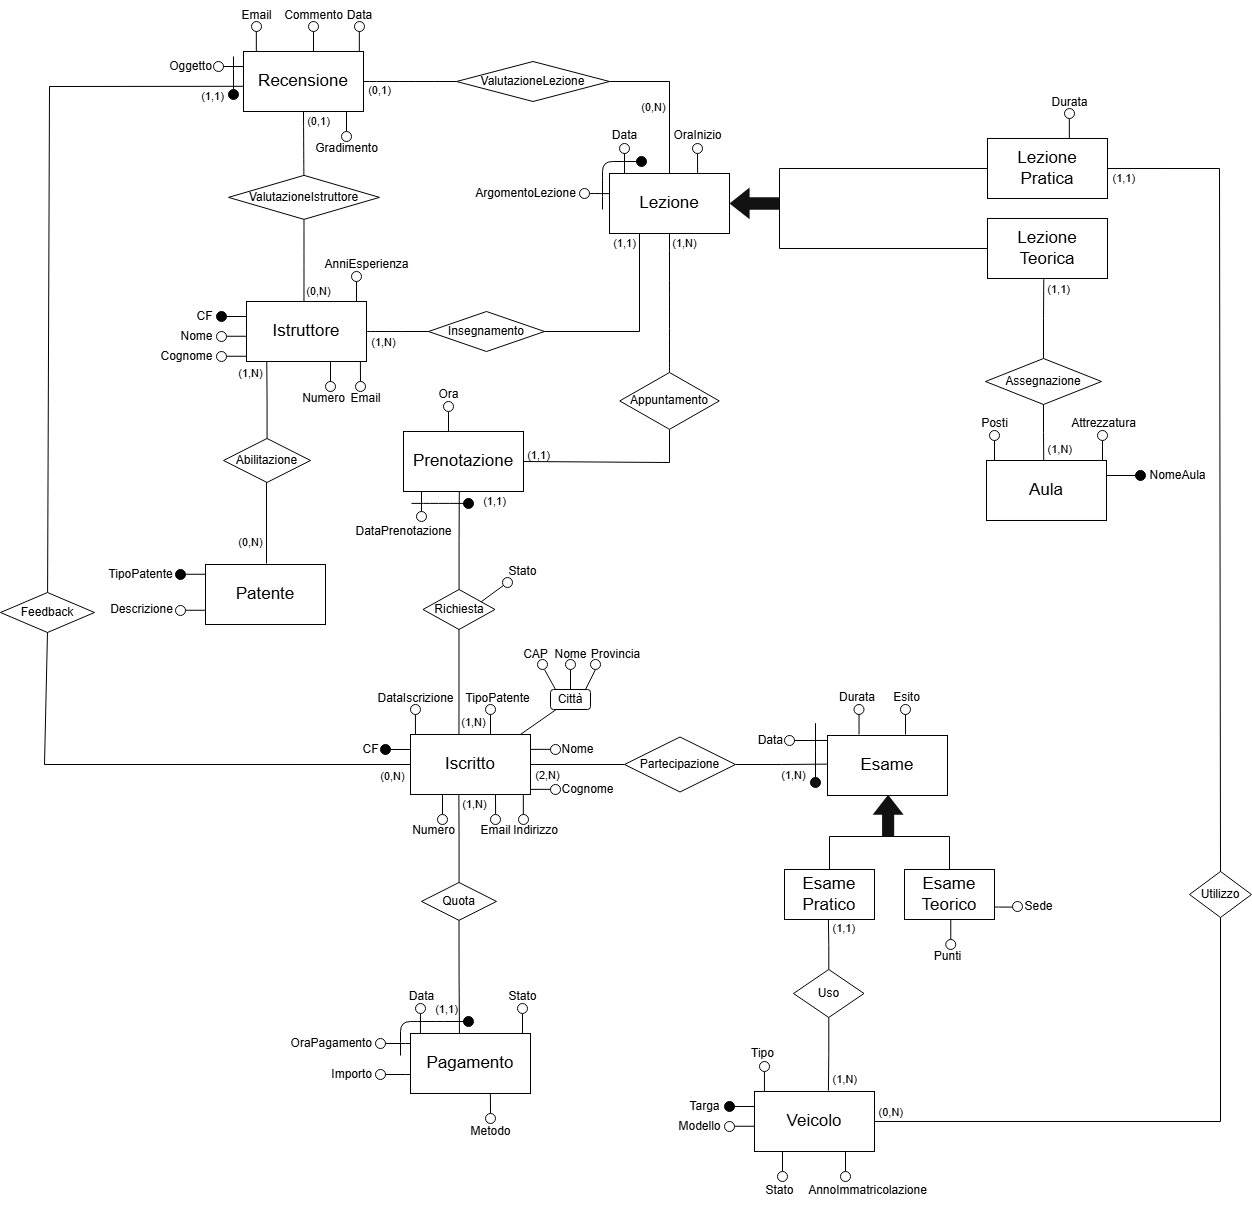
\includegraphics[width=.88\linewidth]{img/ER_ScuolaGuida.drawio.png}\centering
    \caption{Diagramma E-R della base di dati relativa alla gestione di una Scuola Guida}
    \label{fig:diagrammaER}
\end{figure}



\section{Progettazione Logica}{
    In questa sezione viene presentato lo schema logico relazionale derivato dal modello concettuale;
    
    Ciascuna entità concettuale è trasformata in una tabella, definendo attributi, chiavi primarie e chiavi esterne per rappresentare i legami. \\
    Verrà effettuata una analisi degli attributi ridondanti per determinare la loro rimozione o mantenimento al fine per migliorare l’efficienza di archiviazione e accesso.
    
    Le due generalizzazioni concettuali verranno risolte mediante l’introduzione di un attributo discriminante che distingue i tipi di istanza, con i campi specifici resi NULLABLE.
    L'attributo composto "Città" viene reso una tabella a se stante e suddiviso in tre attributi distinti: CAP, Provincia e Nome, per facilitare la gestione dei dati.

    Infine viene riportato il diagramma Entità-Relazione (E-R) ristrutturato, che riporta le modifiche apportate in questa sezione al fine di avere un modello logico completo e coerente.

     \begin{table}[H]
        \centering
        \begin{tabularx}{\textwidth}{|>{\centering\arraybackslash}p{2.6cm}|>{\centering\arraybackslash}X|>{\centering\arraybackslash}p{4.85cm}|>{\centering\arraybackslash}X|}
            \hline
            \rowcolor{lightgray!40}
            \textbf{Entità} & \textbf{Descrizione} & \textbf{Attributi} & \textbf{Identificatore} \\
            \hline
            \rowcolor{white!40}
            Iscritto & Iscritto alla scuola guida & \textit{CF, DataIscrizione, TipoPatente, Città(CAP, Provincia, Nome), Numero, Email, Indirizzo, Cognome, Nome} & \textit{CF}\\
            \hline
            \rowcolor{white!40}
            Istruttore & Istruttore pratico e teorico della scuola guida & \textit{CF, Nome, Cognome, Numero, Email, Abilitazione, AnniEsperienza} & \textit{CF} \\
            \hline
            \rowcolor{white!40}
            Patente & Patente per l'abilitazione & \textit{TipoPatente, Descrizione} & \textit{TipoPatente}, relazione "Abilitazione"\\
            \hline
            \rowcolor{white!40}
            Veicolo & Veicolo utilizzato per esami pratici e lezioni pratiche & \textit{Targa, Modello, Tipo, Stato, AnnoImmatricolazione} & \textit{Targa}\\
            \hline
            \rowcolor{white!40}
            Aula & Aula per le lezioni teoriche & \textit{Nome, Attrezzatura, Posti} & \textit{Nome}\\
            \hline
            \rowcolor{white!40}
            Lezione & Lezione generica & \textit{ArgomentoLezione, Data, OraInizio} & \textit{Data, ArgomentoLezione}\\
            \hline
            \rowcolor{white!40}
            Lezione Teorica & Lezione teorica scuola guida & & \\
            \hline
            \rowcolor{white!40}
            Lezione Pratica & Lezione pratica scuola guida & \textit{Durata} & \\
            \hline
            \rowcolor{white!40}
            Prenotazione & Prenotazione lezioni & \textit{Ora, DataPrenotazione} & \textit{DataPrenotazione}, relazione "Richiesta"\\
            \hline
            \rowcolor{white!40}
            Esame & Esame generico & \textit{Data, Esito, Durata} & \textit{Data}, relazione "Partecipazione"\\
            \hline
            \rowcolor{white!40}
            Esame Teorico & Esame teorico con quiz & \textit{Sede, Punti} & \\
            \hline
            \rowcolor{white!40}
            Esame Pratico & Esame pratico con prova di guida & & \\
            \hline
            \rowcolor{white!40}
            Recensione & Recensione istruttori e lezioni & \textit{Oggetto, Email, Commento, Data, Gradimento} & \textit{Oggetto}, relazione "Feedback"\\
            \hline
            \rowcolor{white!40}
            Pagamento & Pagamenti associati ai servizi offerti & \textit{Importo, Data, Stato, Metodo} & \textit{Importo, Data}, relazione "Quota"\\
            \hline
        \end{tabularx}
        \caption{Entità}
        \label{fig:tabellaEntita}
    \end{table}

    \newpage

    \begin{table}[H]
        \centering
        \begin{tabularx}{\textwidth}{|>{\centering\arraybackslash}p{3cm}|>{\centering\arraybackslash}X|>{\centering\arraybackslash}p{4.85cm}|>{\centering\arraybackslash}X|}
            \hline
            \rowcolor{lightgray!40}
            \textbf{Relazione} & \textbf{Descrizione} & \textbf{Componente} & \textbf{Attributi} \\
            \hline
            \rowcolor{white!40}
            Feedback & Feedback di un iscritto & Iscritto, Recensione & \\
            \hline
            \rowcolor{white!40}
            ValutazioneIstruttore & Recensione di un iscrittore & Recensione, Istruttore & \\
            \hline
            \rowcolor{white!40}
            ValutazioneLezione & Recensione di una lezione & Recensione, Lezione & \\
            \hline
            \rowcolor{white!40}
            Abilitazione & Abilitazione di un istruttore per una patente & Istruttore, Patente & \\
            \hline
            \rowcolor{white!40}
            Insegnamento & Svolgimento della lezione da parte di un istruttore & Istruttore, Lezione & \\
            \hline
            \rowcolor{white!40}
            Appuntamento & Prenotazione di una lezione & Prenotazione, Lezione & \\
            \hline
            \rowcolor{white!40}
            Richiesta & Richiesta di un iscritto per una prenotazione & Iscritto, Prenotazione & \textit{stato}\\
            \hline
            \rowcolor{white!40}
            Partecipazione & Iscrizione ad un esame di un iscritto & Esame, Iscritto & \\
            \hline
            \rowcolor{white!40}
            Quota & Versamento di una quota da parte di un iscritto & Iscritto, Pagamento & \\
            \hline
            \rowcolor{white!40}
            Uso & Utilizzo di un veicolo per un esame pratico & Esame Pratico, Veicolo& \\
            \hline
            \rowcolor{white!40}
            Utilizzo & Utilizzo di un veicolo per una lezione pratica & Veicolo, Lezione Pratica & \\
            \hline
            \rowcolor{white!40}
            Assegnazione & Aula usata per una lezione teorica & Aula, Lezione Teorica & \\
            \hline
        \end{tabularx}
        \caption{Relazioni}
        \label{fig:tabellaRelazioni}
    \end{table}

    \subsection{Analisi delle ridondanze}{
        L’attributo \textit{Email} presente in Recensione, che memorizza l’indirizzo email dell’iscritto autore della recensione, presenta una ridondanza. Questo valore può infatti essere ottenuto tramite la relazione con l’entità Iscritto, accedendo all’attributo Email già presente lì.

        Questo attributo viene modificato ogni volta che un iscritto aggiorna i propri dati anagrafici (evento poco frequente), ma viene visualizzato frequentemente, ad esempio ogni volta che un amministratore consulta le recensioni lasciate dagli utenti.
        Si stima che vengano inserite circa 60 recensioni nuove a settimana, mentre la lettura delle recensioni avviene in media 200 volte a settimana da parte del personale o dei sistemi di report.
        Questo si riassume nelle seguenti due operazioni:
        \begin{itemize}
            \item \textbf{Operazione 1 (60 a settimana)} : Memorizza 60 nuove recensioni nella tabella Recensione.
            \item \textbf{Operazione 2 (200 a settimana)} : Visualizza l’indirizzo email associato a una determinata recensione (ad esempio in fase di moderazione o gestione del feedback da parte dell'amministrazione).
        \end{itemize}

        Assumendo i seguenti volumi nella base di dati:

        \begin{table}[H]
            \centering
            \begin{tabular}{|>{\centering\arraybackslash}p{2.6cm}|>{\centering\arraybackslash}p{2cm}|>{\centering\arraybackslash}p{3cm}|}
                \hline
                \rowcolor{lightgray!40}
                \textbf{Concetto} & \textbf{Costrutto} & \textbf{Volume} \\
                \hline
                \rowcolor{white!40}
                Iscritto & E & 1000\\
                \hline
                \rowcolor{white!40}
                Recensione & E & 3000\\
                \hline
            \end{tabular}
        \end{table}
        
        la seguente analisi serve per stabilire se sia utile o meno tenere l’attributo ridondante
        \textit{Email} in Recensioni. \\

        \textbf{CON RIDONDANZA}: Analizziamo prima il costo totale con ridondanza:
        \begin{itemize}
            \item \textbf{Operazione 1}:
        
            \noindent
            \begin{minipage}[t]{0.7\textwidth}
                \vspace{0pt}
                \begin{tabular}{|>{\centering\arraybackslash}p{2.6cm}|
                                >{\centering\arraybackslash}p{2cm}|
                                >{\centering\arraybackslash}p{3cm}|
                                >{\centering\arraybackslash}p{2cm}|}
                    \hline
                    \rowcolor{lightgray!40}
                    \textbf{Concetto} & \textbf{Costrutto} & \textbf{Accessi} & \textbf{Tipo} \\
                    \hline
                    \rowcolor{white!40}
                    Recensione & E & 1 & S \\
                    \hline
                    \rowcolor{white!40}
                    Iscritto & E & 1 & L \\
                    \hline
                \end{tabular}
            \end{minipage}%
            \begin{minipage}[t]{0.4\textwidth}
                \vspace{3.5ex} % allineamento verticale alla prima riga della tabella
                \begin{flushleft}
                    $\times\ 60$ \\
                    $\times\ 60$ \\
                \end{flushleft}
            \end{minipage}
        
            \vspace{1em}
        
            \item \textbf{Operazione 2}:
        
            \noindent
            \begin{minipage}[t]{0.7\textwidth}
                \vspace{0pt}
                \begin{tabular}{|>{\centering\arraybackslash}p{2.6cm}|
                                >{\centering\arraybackslash}p{2cm}|
                                >{\centering\arraybackslash}p{3cm}|
                                >{\centering\arraybackslash}p{2cm}|}
                    \hline
                    \rowcolor{lightgray!40}
                    \textbf{Concetto} & \textbf{Costrutto} & \textbf{Accessi} & \textbf{Tipo} \\
                    \hline
                    \rowcolor{white!40}
                    Recensione & E & 1 & L \\
                    \hline
                \end{tabular}
            \end{minipage}%
            \begin{minipage}[t]{0.2\textwidth}
                \vspace{3.5ex}
                \begin{flushleft}
                    $\times\ 200$
                \end{flushleft}
            \end{minipage}
        \end{itemize}
        
        \vspace{1em}
        
        Assumendo \textit{costo doppio per gli accessi in scrittura}, il costo totale è:
        \[
            \text{Costo Totale} = 60 \times 2 + 60 + 200 = \boxed{380}
        \]
        
        \textbf{SENZA RIDONDANZA}: Analizziamo il costo totale senza ridondanza:
        \begin{itemize}
            \item \textbf{Operazione 1}:
        
            \noindent
            \begin{minipage}[t]{0.7\textwidth}
                \vspace{0pt}
                \begin{tabular}{|>{\centering\arraybackslash}p{2.6cm}|
                                >{\centering\arraybackslash}p{2cm}|
                                >{\centering\arraybackslash}p{3cm}|
                                >{\centering\arraybackslash}p{2cm}|}
                    \hline
                    \rowcolor{lightgray!40}
                    \textbf{Concetto} & \textbf{Costrutto} & \textbf{Accessi} & \textbf{Tipo} \\
                    \hline
                    \rowcolor{white!40}
                    Recensione & E & 1 & S \\
                    \hline
                \end{tabular}
            \end{minipage}%
            \begin{minipage}[t]{0.4\textwidth}
                \vspace{3.5ex} % allineamento verticale alla prima riga della tabella
                \begin{flushleft}
                    $\times\ 60$ \\
                \end{flushleft}
            \end{minipage}

            Nessun accesso aggiuntivo per aggiornare \textit{Email}, in quanto non viene salvato. \\
            
            \vspace{1em}
        
            \item \textbf{Operazione 2}:
                    
            \noindent
            \begin{minipage}[t]{0.7\textwidth}
                \vspace{0pt}
                \begin{tabular}{|>{\centering\arraybackslash}p{2.6cm}|
                                >{\centering\arraybackslash}p{2cm}|
                                >{\centering\arraybackslash}p{3cm}|
                                >{\centering\arraybackslash}p{2cm}|}
                    \hline
                    \rowcolor{lightgray!40}
                    \textbf{Concetto} & \textbf{Costrutto} & \textbf{Accessi} & \textbf{Tipo} \\
                    \hline
                    \rowcolor{white!40}
                    Recensione & E & 1 & L \\
                    \hline
                    \rowcolor{white!40} 
                    Iscritto & E & 1 & L \\
                    \hline
                \end{tabular}
            \end{minipage}%
            \begin{minipage}[t]{0.2\textwidth}
                \vspace{3.5ex}
                \begin{flushleft}
                    $\times\ 200$ \\
                    $\times\ 200$ \\
                \end{flushleft}
            \end{minipage}
        \end{itemize}
        
        \vspace{1em}
        
        Assumendo \textit{costo doppio per gli accessi in scrittura}, il costo totale è:
        \[
            \text{Costo Totale} = 60 \times 2 + 200 \times 2 = \boxed{520}
        \]

        L’analisi suggerisce quindi di tenere l’attributo ridondante, ottimizzando cosi' il
        numero di accessi.
    }
    \subsection{Eliminazione delle generalizzazioni}{
        Le generalizzazioni descritte in \hyperref[sec:progettazioneConcettuale]{Sezione~\ref*{sec:progettazioneConcettuale}} vengono 
        eliminate attraverso una ristrutturazione dello schema concettuale, 
        con l’obiettivo di semplificare la successiva implementazione del modello relazionale 
        e ridurre la presenza di valori NULL. \\
        Le modifiche vengono applicate come segue:
        \begin{itemize}
            \item \textbf{Lezione} \\ La generalizzazione totale ed esclusiva di LEZIONE viene rimossa 
            accorpando le entità figlie Lezione Teorica e Lezione Pratica all'interno dell'entità 
            padre, come mostrato in \hyperref[fig:diagrammaERristrutturato]{Figura~\ref*{fig:diagrammaERristrutturato}}.
            Questa scelta semplifica la struttura del modello 
            e permette di distinguere i due tipi di lezione attraverso un apposito attributo 
            discriminante Tipo, che ne indica la natura teorica o pratica. \\
            Inoltre, l’attributo proprio \textit{Durata}, specifico delle sole lezioni pratiche, 
            viene incluso direttamente in 
            Lezione come campo NULLABLE, evitando così la creazione di entità separate. \\
            Se si fosse mantenuta un’unica entità Lezione con tutti gli attributi relativi a 
            entrambe le sottoclassi senza distinguere i casi, le lezioni teoriche avrebbero 
            presentato campi nulli come \textit{Durata}, mentre le lezioni pratiche non avrebbero 
            utilizzato altri attributi eventualmente specifici delle lezioni teoriche (come \textit{Aula}). \\
            Separando logicamente i due casi tramite l’attributo \textit{TipoLezione} e rendendo \textit{Durata} 
            facoltativo, si garantisce che ogni istanza contenga solo le informazioni rilevanti.
            In questa soluzione, coerentemente con la metodologia vista a lezione, 
            non sono presenti entità figlie autonome e l’identificazione avviene direttamente 
            tramite i campi della superclasse. \\
            Sarebbe stato possibile mantenere le entità figlie,
            spostando in esse gli attributi specifici, ma ciò avrebbe comportato la duplicazione 
            delle relazioni comuni come Prenotazione e Recensione verso entrambe
            le sottoclassi.
            \item \textbf{Esame} \\In maniera simile, la generalizzazione totale ed esclusiva di ESAME viene sostituita 
            accorpando le entità figlie all’interno dell'entità padre, come mostrato in \hyperref[fig:diagrammaERristrutturato]{Figura~\ref*{fig:diagrammaERristrutturato}}. \\ 
            Anche in questo caso, seguendo un ragionamento simile a quello fatto per la 
            generalizzazione precedente, questo cambiamento consente la riduzione di valori nulli.
            Essendo la generalizzazione totale (ogni esame è necessariamente teorico o pratico), 
            la soluzione di eliminare l’entità padre Esame non sarebbe corretta. \\
            L'integrazione avviene mediante l'inclusione degli attributi propri delle sottoclassi,
            come ad esempio \textit{Punti} e \textit{Sede} dell'esame teorico, direttamente in Esame come campi 
            NULLABLE, distinguendo i due casi attraverso un attributo discriminante \textit{TipoEsame}. \\
            Questo consente di rappresentare le informazioni in modo compatto e coerente, 
            evitando la duplicazione di relazioni comuni come quella con Iscritto.
        \end{itemize}
    }

    \subsection{Scelta di identificatori primari}{
        In questa sezione si analizzano le entità e le relazioni per determinare se sia opportuno partizionare o accorpare alcune di esse:\\
        \\ \textbf{Città.} \\ 
        Creiamo quindi una ulteriore entità Città partendo dall'attributo composto \textit{Città} che contiene gli attributi: \textit{CAP, Provincia e NomeCittà}.
    }

    \subsection{Partizionamento/Accorpamento di Entitá e Relationships}{
        Alla nuova entitá cittá viene aggiunto l’attributo \href{https://www.agenziaentrate.gov.it/portale/documents/20143/448384/Tabella+codici+catastali+comuni_T4_codicicatastali_comuni_24_05_2019.pdf/d4fa70bd-f4bd-caba-24cb-5cc3611237c0}{\textit{CodiceCatastale}} anche noto come “codice
        Belfiore” che identifica univocamente ogni comune nei registri catastali.
    }

    \newpage

    \begin{figure}[H]        
        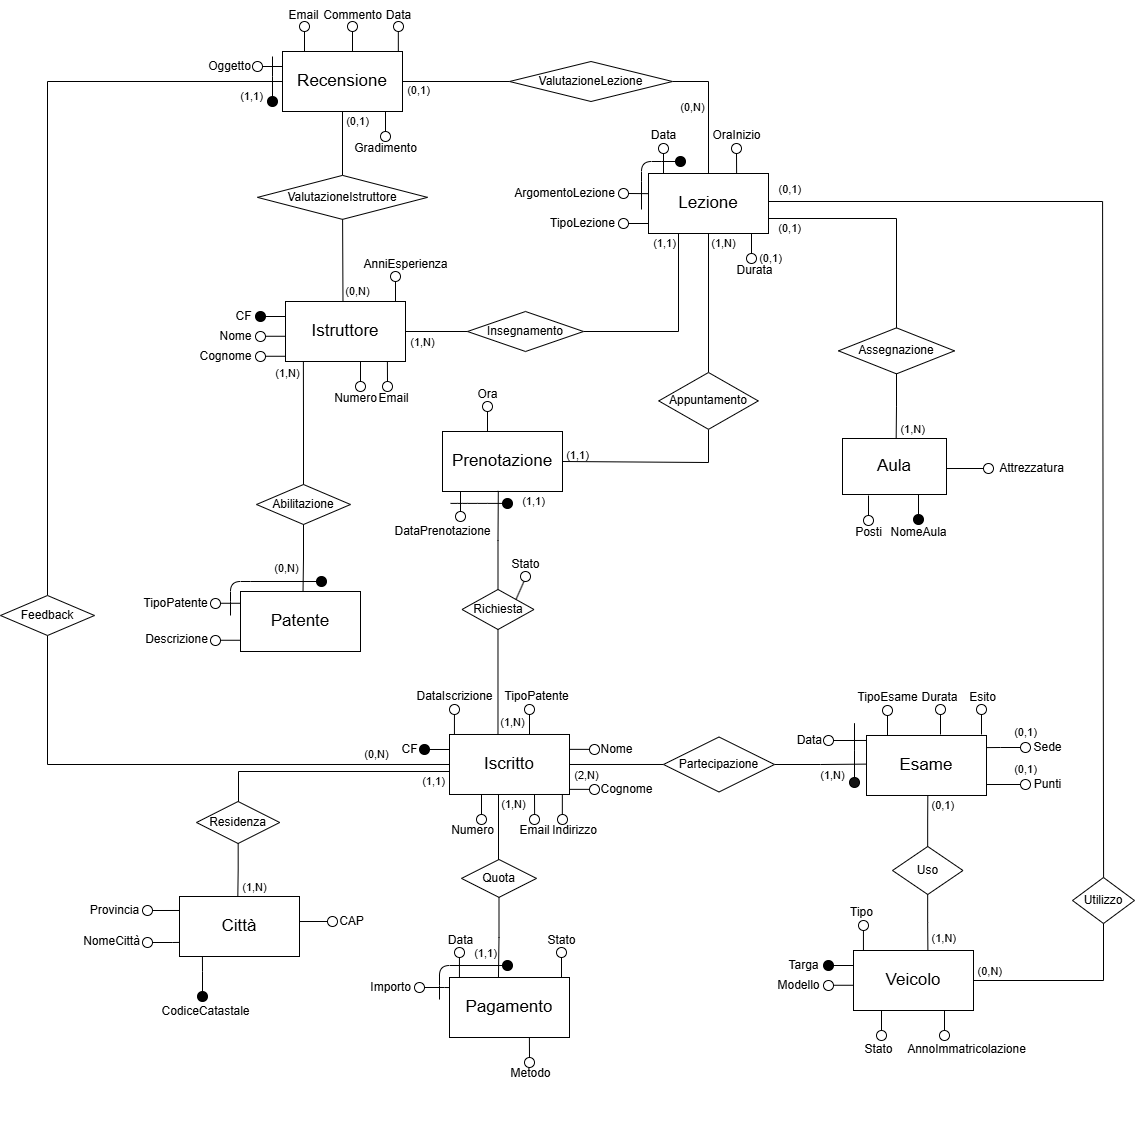
\includegraphics[width=1\linewidth]{img/ER_ScuolaGuidaRistrutturato.drawio.png}\centering
        \caption{Diagramma E-R Ristrutturato}
        \label{fig:diagrammaERristrutturato}
    \end{figure}

    \subsection{Schema Relazionale}{
        Lo schema ristrutturato in \hyperref[sec:progettazioneConcettuale]{Figura~\ref*{sec:progettazioneConcettuale}} contiene solamente costrutti mappabili in corrispettivi dello schema relazionale - detto anche schema logico. Lo schema logico è rappresentato a seguire, dove l’asterisco dopo il nome degli attributi indica quelli che ammettono valori nulli.

        \begin{itemize}
            \item \textbf{Lezione}(\underline{ArgomentoLezione, Data}, OraInizio, Tipo, Durata*, CFIstruttore, IDAula)
            \begin{itemize}
                \item Lezione.CFIstruttore  $\rightarrow$ Istruttore.CF
                \item Lezione.IDAula  $\rightarrow$ Aula.Nome
            \end{itemize}
            \item \textbf{Iscritto}(\underline{CF}, DataIscrizione, TipoPatente, Numero, Email, Indirizzo, Cognome, Nome, idCittà)
            \begin{itemize}
                \item Iscritto.idCittà $\rightarrow$ Città.CodiceCatastale
            \end{itemize}
            \item \textbf{Città}(\underline{CodiceCatastale}, NomeCittà, Provincia, CAP)
            \item \textbf{Istruttore}(\underline{Nome}, Attrezzatura, Posti)
            \item \textbf{Patente}(\underline{TipoPatente, Istruttore}, Descrizione)
            \begin{itemize}
                \item Patente.Istruttore → Istruttore.CF
            \end{itemize}
            \item \textbf{Veicolo}(\underline{Targa}, Modello, Tipo, Stato, AnnoImmatricolazione)
            \item \textbf{Aula}(\underline{Nome}, Attrezzatura, Posti)
            \item \textbf{Prenotazione}(\underline{DataPrenotazione, Iscritto}, Email)
            \begin{itemize}
                \item Prenotazione.Iscritto → Iscritto.CF
                \item Prenotazione.IDLezione → Lezione.(ArgomentoLezione, Data)
            \end{itemize}
            \item \textbf{Esame}(\underline{Data, Iscritto}, Esito, Durata, Tipo, Sede*, Punti*)
            \begin{itemize}
                \item Esame.Iscritto → Iscritto.CF
            \end{itemize}
            \item \textbf{Recensione}(\underline{Oggetto, Iscritto}, Email, Commento, Data, Gradimento)
            \begin{itemize}
                \item Recensione.Iscritto $\rightarrow$ Iscritto.CF
            \end{itemize}
            \item \textbf{Pagamento}(\underline{Importo}, Data, Stato, Metodo, Iscritto)
            \begin{itemize}
                \item Pagamento.Iscritto $\rightarrow$ Iscritto.CF
            \end{itemize}
            \item \textbf{Partecipazione}(\underline{PersonaCF, DataEsame})
            \begin{itemize}
                \item Partecipazione.PersonaCF $\rightarrow$ Iscritto.CF
                \item Partecipazione.DataEsame $\rightarrow$ Esame.Data
            \end{itemize}
            \item \textbf{Abilitazione}(\underline{IstruttoreCF, TipoPatente})
            \begin{itemize}
                \item Abilitazione.IstruttoreCF $\rightarrow$ Istruttore.CF
                \item Abilitazione.TipoPatente $\rightarrow$ Patente.TipoPatente
            \end{itemize}
        \end{itemize}
    }
}

\section{Implementazione in PostgreSQL e Definizione
delle Query}{
    Il file ScuolaGuida.sql contiene il codice SQL necessario per la creazione e il popolamento delle tabelle del database. Questo file include inoltre una serie di query per l’estrazione dei dati e un indice creato specificamente per migliorare le prestazioni
    di una di queste interrogazioni.

    \subsection{Definizione delle query}{
        Di seguito vengono presentate e descritte le query con i relativi output generati e viene motivato l’utilizzo dell’indice proposto. 

        \noindent \textbf{Query 1} Calcolare, per ogni tipo di patente, il numero di esami teorici sostenuti, la media dei punti ottenuti e i promossi, considerando solo chi ha ottenuto in media più di 20 punti. I risultati sono ordinati per media punti in modo decrescente.

        $$
            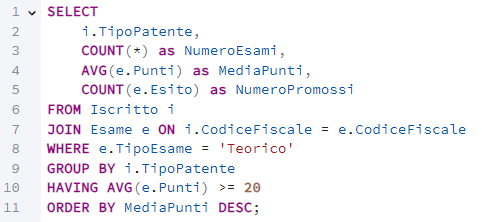
\includegraphics[width=.5\linewidth]{img/query1.png}
        $$

        Un estratto dell'output: 

        $$
            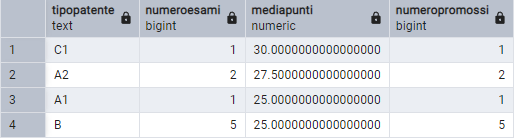
\includegraphics[width=.6\linewidth]{img/risultati1.png}
        $$

        \noindent \textbf{Query 2} Analizzare i veicoli per tipo, conteggiando il numero totale, quelli disponibili, i tipi di patente necessari e le prenotazioni effettuate. I dati sono raggruppati per tipo di veicolo e ordinati per numero di veicoli decrescente.

        $$
            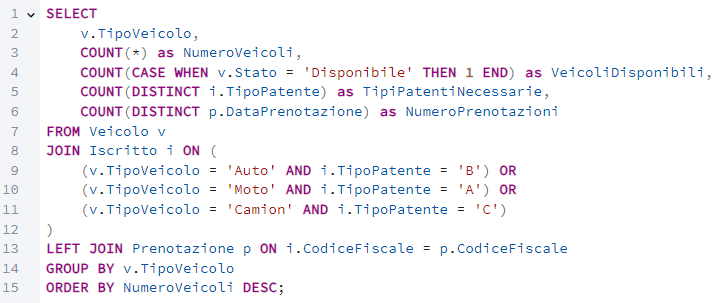
\includegraphics[width=.55\linewidth]{img/query2.png}
        $$

        Un estratto dell'output: 

        $$
            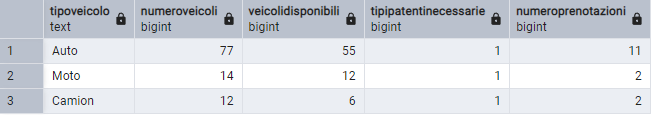
\includegraphics[width=.6\linewidth]{img/risultati2.png}
        $$

        \noindent \textbf{Query 3} Visualizzare le prenotazioni accettate per veicoli disponibili, mostrando data, ora, modello, stato del veicolo e dati dell’iscritto. I risultati sono ordinati cronologicamente per data e ora della prenotazione.

        $$
            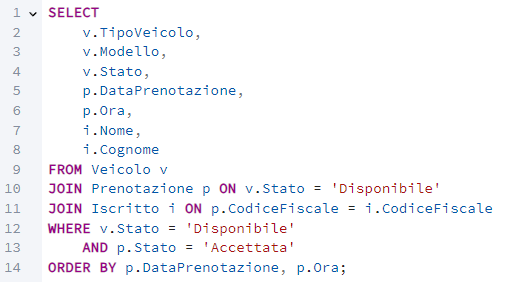
\includegraphics[width=.55\linewidth]{img/query3.png}
        $$

        Un estratto dell'output: 

        $$
            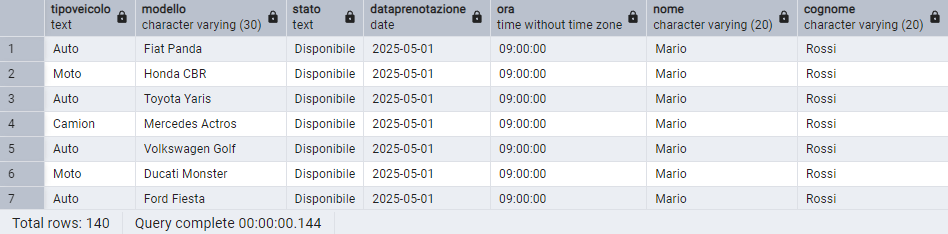
\includegraphics[width=.65\linewidth]{img/risultati3.png}
        $$

        \noindent \textbf{Query 4} Elencare le aule dotate di attrezzatura moderna (Proiettore o LIM), indicando numero di studenti, argomenti trattati, prima e ultima lezione teorica. Le aule sono ordinate per numero di studenti in ordine decrescente.

        $$
            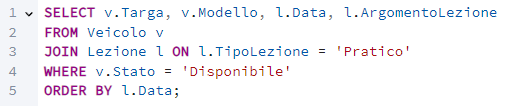
\includegraphics[width=.5\linewidth]{img/query4.png}
        $$

        Un estratto dell'output: 

        $$
            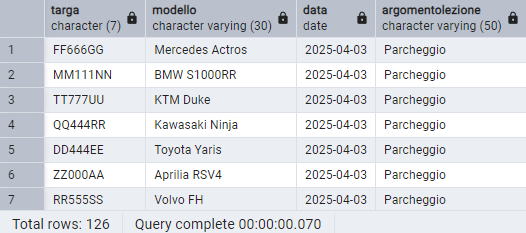
\includegraphics[width=.65\linewidth]{img/risultati4.png}
        $$

        \noindent \textbf{Query 5} Calcolare, per ogni istruttore, la media di gradimento ricevuta e il numero di recensioni scritte da iscritti. Vengono mostrati solo gli istruttori con una media di gradimento superiore a 4.

        $$
            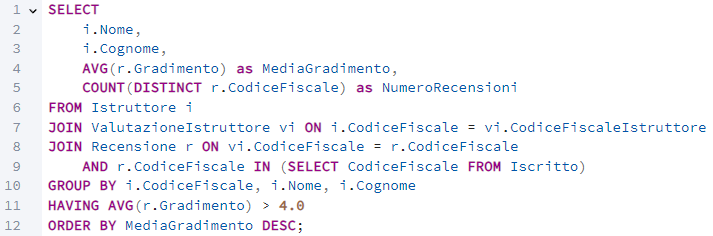
\includegraphics[width=.6\linewidth]{img/query5.png}
        $$

        Un estratto dell'output: 

        $$
            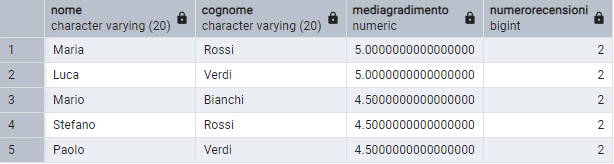
\includegraphics[width=.6\linewidth]{img/risultati5.png}
        $$
    }

}

\end{document}